\documentclass{bmvc2k}

\usepackage{amsmath}
\usepackage{relsize}
\usepackage{algorithm}
\usepackage{algpseudocode}
\usepackage{multirow}
\usepackage{tikz}
\usetikzlibrary{matrix,chains,positioning,decorations.pathreplacing,arrows}

\DeclareMathOperator*{\argmax}{arg\,max}
\DeclareMathOperator*{\argmin}{arg\,min}


%% Enter your paper number here for the review copy
% \bmvcreviewcopy{??}

\title{CT-DANN: Co-teaching Meets DANN for Wild Unsupervised Domain Adaptation}

% Enter the paper's authors in order
% \addauthor{Name}{email/homepage}{INSTITUTION_CODE}
\addauthor{Rahul Bansal\\Sr No. 04-03-02-10-42-18-1-15793}{rahulbansal@iisc.ac.in}{1}
%\addauthor{Petra Prof}{http://www.vision.inst.ac.uk/~pp}{1}
%\addauthor{Colin Collaborator}{colin@collaborators.com}{2}

% Enter the institutions
% \addinstitution{Name\\Address}
\addinstitution{
 Advised by Prof. Soma Biswas\\
 IACV Lab, IISc Bangalore
}
%\addinstitution{
% Collaborators, Inc.\\
% 123 Park Avenue,\\
% New York, USA
%}

% \runninghead{Student, Prof, Collaborator}{BMVC Author Guidelines}

% Any macro definitions you would like to include
% These are not defined in the style file, because they don't begin
% with \bmva, so they might conflict with the user's own macros.
% The \bmvaOneDot macro adds a full stop unless there is one in the
% text already.
\def\eg{\emph{e.g}\bmvaOneDot}
\def\Eg{\emph{E.g}\bmvaOneDot}
\def\etal{\emph{et al}\bmvaOneDot}

%------------------------------------------------------------------------- 
% Document starts here
\begin{document}
\maketitle
\begin{abstract} 
Domain adaptation learns the task for unlabeled target domain data by knowledge transfer from a source domain with rich annotations. It is not uncommon that “source-domain engineering” becomes a cumbersome process in domain adaptation: the high-quality source domains highly related to the target domain are hardly available.  Here, we consider a new, more realistic and more challenging problem setting, where model has to be trained with noisy labeled data from source domain and unlabeled data from target data; named weak or wild unsupervised domain adaptation(WUDA). Running standard domain adaptation netowork in WUDA setting results in severe negative transfer from noisy source domain. Co-teaching is one of the state of the art of the method in learning classifiers from noisy data. In this work, we incorporate co-teaching framework in standard domain adaptation network to train model using noisy source data and unlabeled target data. Here, we propose end to end deep neural architecture incorporating co-teaching framework in standard domain adaptation network. By extensive experiments, we show that our approach eliminates the negative transfer from noisy source data.
\end{abstract}
\section{Introduction}
The immense success of deep learning networks depends upon the availability of well-annotated training datasets on the domains of the tasks of interest. 
%Deep learning networks have shown significant advancement in the field of computer vision with image classification\cite{imagenet} as one of the prominent examples. A key factor to achieve such advancements is the availability of well-annotated training datasets on the domains of the tasks of interest. 
However, such annotations can be overly expensive to attain for the amount of data required for plausible performance by today’s deep neural networks. 
Domain adaptation approaches attempt to compensate for lack of annotated data in a \textit{target domain}, by leveraging information from a \textit{source domain}, for which annotated data is easier to obtain. 
Domain adaptation (DA) aims to learn domain invariant features which are discriminative in nature, so that task classifiers learned from the source data can be readily applied to the target domain~\cite{uda,dann,ctc,ltdan,atda,saito2017maximum}.
Existing unsupervised DA (UDA) approaches assume that the source domain has clean labeled data training data, while the target data is unlabeled. 
This is a restrictive assumption, since source domain data is usually collected from crowd sourcing platform or crawling through the Internet making their labels noisy and not completely reliable.

In this work, we address the more realistic and significantly more challenging wildy unsupervised domain adaptation (WUDA) [][], which aims to transfer knowledge from noisy labeled data in source domain ($\tilde{P_s}$, i.e., noisy source data) to unlabeled target data ($P_{x_{t}}$).
This is a relatively unexplored area and it is only recently that researchers have started to address this problem[].
%Unfortunately, existing DA methods share an implicit assumption that there are no noisy source data. Namely, these methods focus on transferring knowledge from clean source data ($P_s$) to unlabeled target data ($P_{x_{t}}$).\\
A naive approach to handle WUDA is to directly apply standard UDA methods, which will simply match the target domain with the entire noisy
source domain, resulting in severe negative transfer and performance degradation. 

In this work, we propose a novel approach to address the WUDA task, which aims to select clean instances from the noisy source samples and use these samples to update the domain adaptation model. 
The bottleneck is how to select the clean instances out of noisy instances?
Inspired by the success of the small-loss clean sample selection approaches, we incorporate one of the state-of-the-art model \textit{Co-teaching}\cite{coteaching} in \textit{domain-adversarial neural network} (DANN)\cite{dann}. 
Co-teaching addresses the task of image classification under noisy labels, is based on the study that deep models can memorize easy instances first, and gradually adapt to hard instances as training epochs become large~\cite{memorization}. 
It trains two networks in parallel and updates the weights of the networks using only the small loss samples and the gradients of the two networks are switched during the parameter update. 
Our proposed method worked as a plug in for standard adversarial domain adaptation methods.
As in standard adversarial DA, there are mainly two losses: classification loss (to learn the discriminative features), domain loss (to learn the domain invariant features). and there are three networks $G_f$ ( feature extractor), $G_d$ (domain discriminator), $G_y$ (classifier). In our proposed method for WUDA, two identical feature extractors are maintained $G_{f}^1$, $G_{f}^2$. Classification loss is calculated only through small loss instances and cross propagated in the peer feature extractor network to update the parameters. However, domain loss is backpropagated as in standard DA using only one feature extractor; say $G_{f_{1}}$.

Extensive experiments and comparisons with the state-of-the-art approaches have been performed on three different datasets, namely Office 31[], Office Home[] with both -- and --- noise labels.
Further, experiments on the Bing Caltech 256 dataset shows the effectiveness of the approach for real noisy data. 


\section{Related Work}

\section{Related Work}
In particular, one common deep solution for unsupervised domain adaptation is to guide the feature learning in DCNNs by minimizing the domain discrepancy with Maximum Mean Discrepancy (MMD). MMD is an effective non-parametric metric for the comparisons between the distributions of source and target domains. \cite{mmd} is one of early works that incorporates MMD into DCNNs with regular supervised classification loss on source domain to learn both semantically meaningful and domain invariant representation. MMD based methods \cite{mmd,ltdan} transfers deep convolutional networks (DCNNs) by adding adaptation layers through which the kernel embeddings of distributions are matched by minimizing MMD. Residual transfer network \cite{rtn} improves the MMD-based methods by adding a shortcut path and adopting entropy minimization criterion. 
Another direction is by exploiting a domain discriminator to distinguish the source and target while learning deep features to confuse the discriminator in an adversarial training paradigm \cite{uda, dann, deeptransfer}.\\
These all methods assume a clean source domain which is limited and expensive in many real-world applications. State-of-the-art domain adaptation methods may suffer from negative transfer caused by noisy source data in wild unsupervised domain adaptation, which will deteriorate the generalization power of networks trained on the noisy source domain when applied to the target domain.\\
Learning discriminative models from datasets with noisy labels is an active area of research. \cite{DBLP:journals/corr/ZhangBHRV16} empirically demonstrated that noisy labels will be memorized by DNNs which destroys their generalization capability. Transferable Curriculum Learning (TCL) \cite{tcl} is one of the state art approach dealing with WUDA setting. Authors in TCL paper used curricum learning \cite{curricumlearn_latent, curricumlearn} which organizes examples in a meaningful order to
promote convergence and optimization. It prioritizes easier examples of smaller loss by
assigning higher weights to them. Different from all previous works, here we incorporate state of the art approach: Co-teaching \cite{coteaching} to learn classifiers from noisy data into standard domain adaptation network. Our aim is to modify the existing standard domain adaptation network to deal with WUDA problem setting also. 
%\subsection{Co-teaching for Handling Label Noise in Image Classification}
Co-teaching~\cite{coteaching} is one of the state-of-the-art approaches for image classification under noisy labels, and can be used to train deep networks robustly even with extremely noisy labels.
It is based on the small-loss concept, i.e. deep models can memorize easy instances first, and gradually adapt to hard instances as training progresses~\cite{memorization}. 
The assumption is that the instances corrupted by label noise are hard for the network to learn, while the clean ones are comparatively easy. 

The Co-teaching algorithm is given in Algorithm \ref{algo:coteaching}.
Specifically, two networks $P$ (with parameter $w^1$) and $Q$ (with parameters $w^2$) are maintained. 
For a mini-batch $\mathcal{D}$ (step 5), the networks $P$ (resp. $Q$) selects a small proportion of instances from this mini-batch $\mathcal{D}^1$ (resp. $\mathcal{D}^2$) that have small training loss (steps 6 and 7). 
The number of instances is controlled by $R(T)$, and $P$ (resp. $Q$) only selects $R(T)$ percentage of small loss instances out of the mini-batch. Then, the selected instances are fed into its peer network as the useful knowledge for parameter updates (steps 8 and 9).
In the training procedure, $R(T)$ is used (at epoch $T$) to quantify the amount of small loss
samples per mini-batch to be used to update the network weights. $R(T)$ is directly related
to the amount of label corruption $\epsilon$ ($\epsilon$ is assumed to be known or estimated), and is defined as $R(T)= 1- \min\bigg\{\dfrac{T}{T_k}\epsilon, \epsilon\bigg\}$, where $T_k$ is the epoch after which $R(T)$ becomes constant. Typical profiles of $R(T)$ for different $\epsilon$ is shown in Figure \ref{fig:R(T)}. 
In Algorithm 1, we observe that the model initially considers all the input data and slowly zones into the cleanly labeled data (guided by the concept of small loss instances) to train the model. After completion of $T_k$ epochs ($T_k$: hyperparameter), the network weights are updated using $(1 - \epsilon)$ portion of the training data (marked as small loss instances) and ignores the large loss samples under the assumption that they are wrongly labeled.
\begin{figure}[ht]
            \centering
            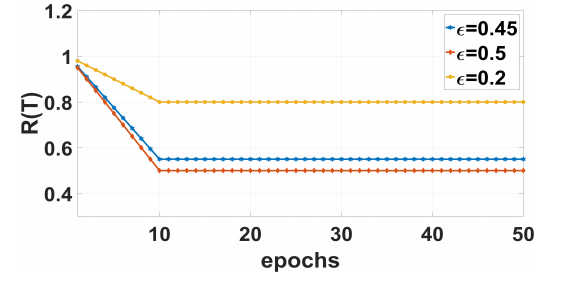
\includegraphics[scale = 0.5]{plot_R(T).png}
            \caption{Plot of $R(T)$ for different values of label corruption $\epsilon =\{0.45,0.5,0.2\}$ and $T_k = 10$. $R(T)$ is used \cite{coteaching} to control how many samples are used to update the network weights per epoch.}
\label{fig:R(T)}
\end{figure}
\begin{algorithm}[H]
	\caption{Co-teaching Algorithm.} 
	\begin{algorithmic}[1]
	    \State \textbf{Input:} $w^1$ and $w^2$, learning rate $\eta$, fixed $\epsilon$, epoch $T_k$ and $T_{max}$, iteration $N_{max}$;
		\For {$T=1,2,\ldots, T_{max}$}
		    \State Training set ${D}$;
			    \For {$N=1,2,\ldots, N_{max}$}
				    \State \textbf{Fetch} mini batch $\mathcal{D}$ from ${D}$
				    \State \textbf{Obtain} $\mathcal{D}^1 = \argmin_{\mathcal{D}':|\mathcal{D}'|\geq R(T)|\mathcal{D}|} \mathcal{L}(P, \mathcal{D}')$   \Comment{$\mathcal{L}$: classification loss}
				    \State \textbf{Obtain} $\mathcal{D}^2 = \argmin_{\mathcal{D}':|\mathcal{D}'|\geq R(T)|\mathcal{D}|} \mathcal{L}(Q, \mathcal{D}')$
				    \State \textbf{Obtain} $L^1(w^1) = \mathcal{L}(P,\mathcal{D}^2)$ \Comment{Loss for network 1: $P$}
				    \State \textbf{Obtain} $L^2(w^2) = \mathcal{L}(Q,\mathcal{D}^1)$ \Comment{Loss for network 2: $Q$}
				    \State \textbf{Update} $w^1 = w^1 - \eta \nabla L^1(w^1)$
				    \State \textbf{Update} $w^2 = w^2 - \eta \nabla L^2(w^2)$
			    \EndFor
			 \State \textbf{Update} $R(T)= 1- \min\bigg\{\dfrac{T}{T_k}\epsilon, \epsilon\bigg\}$
		\EndFor
	\end{algorithmic} 
\label{algo:coteaching}
\end{algorithm}


When the test data follows similar distribution as the training data, Co-teaching will steadily improve learning. 
%However, when the test data has a distribution shift from the training data, the existing curriculum will be less specified. 
But in the problem addressed, due to the distribution shift, the test data will be substantially dissimilar to the training data. 
Thus, even if the training samples with smaller loss are noise-free, they are not necessarily relevant to the learning task of the test data.
\section{Preliminaries}

In this section, first, we formulate the problem of Wild Unsupervised Domain Adaptation (WUDA), and then describe the base networks required to understand the proposed approach.

\subsection{Problem Formulation}
In this work, we are exploring the problem of wild unsupervised domain adaptation(WUDA) in which the target domain is fully unlabeled and the source domain is partially corrupted with label noise. The wild unsupervised domain adaptation scenario constitutes a labeled source domain ${D}_s = \{({x_i}^s, {y_i}^s)\}_{i=1}^{n_s}$ and an unlabeled target domain ${D}_t = \{({x_i}^t)\}_{i=1}^{n_t}$, while the source and target domains follow different distributions $P_s \neq P_t$. Here, we relax the assumptions of clean labels of source domain data.  Our goal is to train a deep network using noisy source data and unlabeled target which generalizes well on target data. Standard DA methods results in severe negative transfer. So we have to modify standard DA methods to eliminate the negative influence of noisy source samples and enable positive transfer of noiseless source samples.

Our aim is to train a deep learning model which is robust to both noisy source samples and distribution shift. 
To address the distribution shift, we use the base network as the domain adversarial neural network (DANN) described below, though other base networks can also be utilised for the same.
To account for the label noise in the source samples, we propose to incorporate a very well established approach for handling noise in image classification network, namely co-teaching framework \cite{coteaching}.
Before we decribe the proposed approach, we will describe the base DANN network and also the co-teaching framework for image classification setup.

\subsection{Base Network - Domain Adversarial Neural Network}
\label{subsec:dann}
Domain adaptation is usually reduced to matching the feature distributions of the source and target domains. In the deep learning regime, this can be done by
learning new feature representations such that the source and target domains
are not distinguishable by a domain discriminator. This idea leads to the a series
of domain adversarial neural networks (DANN)\cite{uda,dann,deeptransfer}, achieving strong performance
in standard domain adaptation with shared label space across domains.
More formally, DANN is a two-player minimax game, where the first player is
a domain discriminator $G_d$ trained to distinguish the source domain from the
target domain, and the second player is a feature extractor $G_f$ simultaneously
trained to confuse the domain discriminator. $G_y$ is the classifier to classify features extracted from $G_f$.
In order to extract domain invariant and discriminant features from $G_f$, the parameters $w_f$ of feature extractor $G_f$ are learnt by maximizing the domain loss and minimizing the classification loss of source domain instances, while the parameters $w_d$ of domain discriminator are learnt by minimizing the domain loss. The parameters $w_y$ of classifier are learnt by minimizing the classification loss of source domain data.
The overall objective of the Domain Adversarial Neural Network (DANN) is
\begin{equation}
\begin{align}
    \mathcal{L}_y(G_f, G_y, D_s)  = \dfrac{1}{n_{s}} \mathlarger\sum\limits_{x_i \in D_s} L_y(G_y(G_f(x_i)),y_i)\\
     \mathcal{L}_d(G_f, G_d, D_s \cup D_t) = \dfrac{1}{n_s + n_t} \sum\limits_{x_i \in {D_s \cup D_t}} L_d(G_d(G_f(x_i)),d_i)\\
     L(w_f, w_y, w_d) = \mathcal{L}_y(G_f, G_y, D_s) - \lambda \mathcal{L}_d(G_f, G_d, D_s \cup D_t)
\end{align}
\end{equation}
$L_y$ and $L_d$ are cross-entropy and binary cross-entropy loss respectively. where $d_i$ is the domain label of $x_i$ , and $\lambda$ is a hyper-parameter to trade off the
two objectives $L_y$ and $L_d$. After training convergence:
\begin{center}
    $\hat{w}_f, \hat{w}_y  = \argmin \limits_{w_f, w_y} L(w_f, w_y, w_d)$\\
    $\hat{w}_d  = \argmax \limits_{w_d} L(w_f, w_y, w_d)$
\end{center}
\subsection{Co-teaching for Handling Label Noise in Image Classification}
Co-teaching~\cite{coteaching} is one of the state-of-the-art approaches for image classification under noisy labels, and can be used to train deep networks robustly even with extremely noisy labels.
It is based on the small-loss concept, i.e. deep models can memorize easy instances first, and gradually adapt to hard instances as training progresses~\cite{memorization}. 
The assumption is that the instances corrupted by label noise are hard for the network to learn, while the clean ones are comparatively easy. 

The Co-teaching algorithm is given in Algorithm \ref{algo:coteaching}.
Specifically, two networks $P$ (with parameter $w^1$) and $Q$ (with parameters $w^2$) are maintained. 
For a mini-batch $\mathcal{D}$ (step 5), the networks $P$ (resp. $Q$) selects a small proportion of instances from this mini-batch $\mathcal{D}^1$ (resp. $\mathcal{D}^2$) that have small training loss (steps 6 and 7). 
The number of instances is controlled by $R(T)$, and $P$ (resp. $Q$) only selects $R(T)$ percentage of small loss instances out of the mini-batch. Then, the selected instances are fed into its peer network as the useful knowledge for parameter updates (steps 8 and 9).
In the training procedure, $R(T)$ is used (at epoch $T$) to quantify the amount of small loss
samples per mini-batch to be used to update the network weights. $R(T)$ is directly related
to the amount of label corruption $\epsilon$ ($\epsilon$ is assumed to be known or estimated), and is defined as $R(T)= 1- \min\bigg\{\dfrac{T}{T_k}\epsilon, \epsilon\bigg\}$, where $T_k$ is the epoch after which $R(T)$ becomes constant. Typical profiles of $R(T)$ for different $\epsilon$ is shown in Figure \ref{fig:R(T)}. 
In Algorithm 1, we observe that the model initially considers all the input data and slowly zones into the cleanly labeled data (guided by the concept of small loss instances) to train the model. After completion of $T_k$ epochs ($T_k$: hyperparameter), the network weights are updated using $(1 - \epsilon)$ portion of the training data (marked as small loss instances) and ignores the large loss samples under the assumption that they are wrongly labeled.
\begin{figure}[ht]
            \centering
            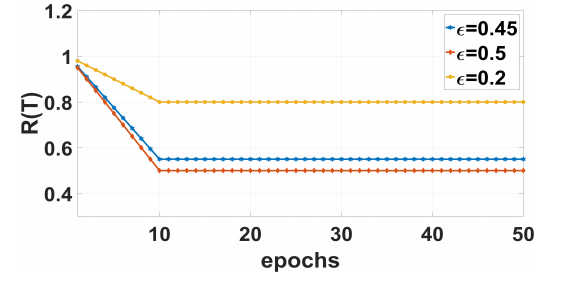
\includegraphics[scale = 0.5]{plot_R(T).png}
            \caption{Plot of $R(T)$ for different values of label corruption $\epsilon =\{0.45,0.5,0.2\}$ and $T_k = 10$. $R(T)$ is used \cite{coteaching} to control how many samples are used to update the network weights per epoch.}
\label{fig:R(T)}
\end{figure}
\begin{algorithm}[H]
	\caption{Co-teaching Algorithm.} 
	\begin{algorithmic}[1]
	    \State \textbf{Input:} $w^1$ and $w^2$, learning rate $\eta$, fixed $\epsilon$, epoch $T_k$ and $T_{max}$, iteration $N_{max}$;
		\For {$T=1,2,\ldots, T_{max}$}
		    \State Training set ${D}$;
			    \For {$N=1,2,\ldots, N_{max}$}
				    \State \textbf{Fetch} mini batch $\mathcal{D}$ from ${D}$
				    \State \textbf{Obtain} $\mathcal{D}^1 = \argmin_{\mathcal{D}':|\mathcal{D}'|\geq R(T)|\mathcal{D}|} \mathcal{L}(P, \mathcal{D}')$   \Comment{$\mathcal{L}$: classification loss}
				    \State \textbf{Obtain} $\mathcal{D}^2 = \argmin_{\mathcal{D}':|\mathcal{D}'|\geq R(T)|\mathcal{D}|} \mathcal{L}(Q, \mathcal{D}')$
				    \State \textbf{Obtain} $L^1(w^1) = \mathcal{L}(P,\mathcal{D}^2)$ \Comment{Loss for network 1: $P$}
				    \State \textbf{Obtain} $L^2(w^2) = \mathcal{L}(Q,\mathcal{D}^1)$ \Comment{Loss for network 2: $Q$}
				    \State \textbf{Update} $w^1 = w^1 - \eta \nabla L^1(w^1)$
				    \State \textbf{Update} $w^2 = w^2 - \eta \nabla L^2(w^2)$
			    \EndFor
			 \State \textbf{Update} $R(T)= 1- \min\bigg\{\dfrac{T}{T_k}\epsilon, \epsilon\bigg\}$
		\EndFor
	\end{algorithmic} 
\label{algo:coteaching}
\end{algorithm}


When the test data follows similar distribution as the training data, Co-teaching will steadily improve learning. 
%However, when the test data has a distribution shift from the training data, the existing curriculum will be less specified. 
But in the problem addressed, due to the distribution shift, the test data will be substantially dissimilar to the training data. 
Thus, even if the training samples with smaller loss are noise-free, they are not necessarily relevant to the learning task of the test data.

% *************************************************************

\section{Proposed CT-DANN for WUDA}
Here, we propose a novel framework, termed CT-DANN, which seamlessly integrates the co-teaching framework with the base DANN for handling noisy data in the source domain as well as the distribution shift between the source and target domain.
A flow-chart of the proposed approach is shown in Figure \ref{flowchart}.
\usetikzlibrary{calc,fit,arrows}
\usetikzlibrary{shapes,arrows,shadows,geometric}
\usetikzlibrary{shapes,shapes.geometric,arrows,fit,calc,positioning,automata}

\tikzstyle{decision} = [diamond, draw, fill=blue!20, 
    text width=4.5em, text badly centered, node distance=3cm, inner sep=0pt]
\tikzstyle{block} = [rectangle, draw, fill=blue!20, 
    text width=2em, text centered,node distance=1.0cm, minimum height=0.5em]
\tikzstyle{line} = [draw, -latex']
\tikzstyle{cloud} = [draw, ellipse,fill=red!20, node distance=3cm,
    minimum height=2em]


    
    
\tikzstyle{input} = [coordinate]
\tikzstyle{container} = [draw, rectangle, dashed, inner sep=1em]

\begin{center}
\begin{figure}[ht]
\scalebox{1.0}{
\begin{tikzpicture}
    % Place nodes
    \centering
    \node [block, fill=blue!20,text width=2em, 
    text centered,node distance=1.0cm, minimum height=0.5em] (f1) {$G_{f}^1$};
    
    \node[inner sep=0,minimum size=0, left of=f1, node distance = 1.2cm] (input1) {}; % invisible node
    
    \node [block, fill=blue!20,text width=2em, 
    text centered,node distance=2.6cm, minimum height=0.5em, right of = f1] (y1) {$G_{y}^1$};
    
    \node [block, fill=blue!20,text width=2em, 
    text centered,node distance=2.2cm, minimum height=0.5em, above of = y1] (d1) {$G_{d}$};
    
    \node [block, fill=blue!20,text width=2em, 
    text centered,node distance=2.0cm, minimum height=0.5em, below of =  f1] (f2) {$G_{f}^2$};
    
    \node[inner sep=0,minimum size=0, left of=f2, node distance = 1.2cm] (input2) {}; % invisible node
    
    \node [block, fill=blue!20,text width=2em, 
    text centered,node distance=2.6cm, minimum height=0.5em, right of = f2] (y2) {$G_{y}^2$};
    
    \path [line] (input1) -- node [text width=2.2cm, midway,above=0.1em] {$\mathcal{D}_s \cup \mathcal{D}_t$} (f1);
    
    \path [line] (input2) -- node [text width=1.2cm, midway,above=0.1em] {$\mathcal{D}_s$} (f2);
    
    \path [line] (f1) -- node [text width=1.1cm, midway,above=0.1em] {$F_{s}^{1} \cup F_{t}^{1}$} (y1);
    
    \node[inner sep=0,minimum size=0, right of=f1, node distance = 0.7cm] (fe1) {}; % invisible node
    
    \node [block, fill=blue!20,text width=1.1em, 
    text centered,node distance=1.0cm, minimum height=0.2em, above of =  fe1] (grl) {grl};
    
    \path [line] (fe1) -- node [text width=2.0cm, midway,above=0.1em] {} (grl);
    
    \path [line] (grl) |- node [text width=2.0cm, midway,above=0.1em] {$F_{s}^{1} \cup F_{t}^{1}$} (d1);
    
    \path [line] (f2) -- node [text width=0.1em, midway,above=0.1em] {$F_{s}^{2}$} (y2);
    
    \node[cloud, fill=blue!20, ellipse , node distance=1.8cm,
    minimum height=2em, right of =  d1] (ld) {$\mathcal{L}_{d}$};
    
    \node[cloud, fill=blue!20, ellipse , node distance=2.0cm,
    minimum height=2em, right of =  y1] (ds1) {$W^1$};
    
    \node[cloud, fill=blue!20, ellipse , node distance=2.0cm,
    minimum height=2em, right of =  y2] (ds2) {$W^2$};
    
    \node[cloud, fill=blue!20, ellipse , node distance=1.6cm,
    minimum height=2em, right of =  ds1] (ly1) {$\mathcal{L}_{y}^1$};
    
    \node[cloud, fill=blue!20, ellipse , node distance=1.6cm,
    minimum height=2em, right of =  ds2] (ly2) {$\mathcal{L}_{y}^2$};
    
    \path [line] (d1) -- node [text width = 0.1em, midway,above=0.1em] {} (ld);
    
    \path [line] (y1) -- node [text width = 0.1em, midway,above=0.1em] {$\hat{Y}_{s}^1$} (ds1);
    
    \path [line] (y2) -- node [text width = 0.1em, midway,below=0.1em] {} (ds2);
    
    
    \path [line] (ds1) -- node [text width = 0.1em, midway,above=0.1em] {} (ly2);
    \path [line] (ds2) -- node [text width = 0.1em, midway,above=0.1em] {} (ly1);
    
    \node[cloud, fill=blue!20, ellipse , node distance=1.6cm,
    minimum height=2em, above of =  ly1] (lt) {$\mathcal{L}_{t}$};
    \node[inner sep=0,minimum size=0, right of=y1, node distance = 0.7cm] (ye1) {}; % invisible node
    \path [line] (ye1) |- node [text width = 0.01em, midway,below=0.1em] {$\hat{Y}_{t}^1$} (lt);
    
    \node [block, draw, fill=white!20,text width=4.0cm,anchor=west, node distance=9.0cm, minimum height=7.5cm, right of = f1] (legend) {$\mathcal{D}_s$: mini-batch source data\\
    $\mathcal{D}_t$: mini-batch target data\\
    $G_{f}^1 + G_{y}^1$ : network 1\\
    $G_{f}^2 + G_{y}^2$ : network 2\\
    $G_f$: feature extractor\\
    $G_y$: feature classifier\\
    grl: gradient reversal layer\\
    $F_s$: features of source data\\
    $F_t$ : features of target data\\
    $\hat{Y}_s$ : source probabilties\\
    $\hat{Y}_t$ : target probabilties\\
    $G_d$: domain discriminator\\
    $\mathcal{L}_y$: classificaton loss\\
    $\mathcal{L}_d$: domain loss\\
    $\mathcal{L}_t$: entropy loss\\
    $\mathcal{D}_{s}^1$ \& $\mathcal{D}_{s}^2$: small loss data
    ^{1,2} \text{ corresponds to network}\\};
    
    
\end{tikzpicture}}
\caption{High level flow diagram}
\label{flowchart}
\end{figure}
\end{center}
\vspace{-1cm}
\usetikzlibrary{calc,fit,arrows}
\usetikzlibrary{shapes,arrows,shadows,geometric}
\usetikzlibrary{shapes,shapes.geometric,arrows,fit,calc,positioning,automata}

\tikzstyle{decision} = [diamond, draw, fill=blue!20, 
    text width=4.5em, text badly centered, node distance=3cm, inner sep=0pt]
\tikzstyle{block} = [rectangle, draw, fill=blue!20, 
    text width=2em, text centered,node distance=1.6cm, minimum height=2em]
\tikzstyle{line} = [draw, -latex']
\tikzstyle{cloud} = [draw, ellipse,fill=red!20, node distance=3cm,
    minimum height=2em]
    
\tikzstyle{input} = [coordinate]
\tikzstyle{container} = [draw, rectangle, dashed, inner sep=1em]




\begin{figure}[ht]
\scalebox{1.0}{
\centering      
\begin{tikzpicture}
    % Place nodes
    \node[inner sep=0,minimum size=0] (inv1) {}; % invisible node

    \node [block, node distance = 3.5cm, right of = inv1] (gf1) {$G_{f}^1$};
    
    \node [block, right of = gf1] (gy1) {$G_{y}^1$};
    
    \node[container, fit=(gf1)(gy1)] (FTCBlockVal) (Blk1){};
    \node at (Blk1.south) [below, node distance = 0.6cm and 0]{Network 1 : $P$};
    
    \node [block, node distance=2.5cm, right of =  gy1] (gf2) {$G_{f}^2$};
    
    \node [block, right of = gf2] (gy2) {$G_{y}^2$};
    
    \node[container, fit=(gf2)(gy2)] (FTCBlockVal) (Blk2){};
    \node at (Blk2.south) [below, node distance = 0.6cm and 0]{Network 2 : $Q$};
    
    
    % Draw edges
    \path [line] (gf1) -- node [] {} (gy1);
    \path [line] (gf2) -- node [] {} (gy2);
    
\end{tikzpicture}}

\caption{Network 1 \& 2 as per co-teaching framework}
\label{fig:networks}
\end{figure}





The proposed CT-DANN consists of two pairs of feature extractors and classifiers, denoted by $(G_{f}^1$ \& $G_{y}^1)$ and $(G_{f}^2$ \& $G_{y}^2)$ having parameters $(w_{f}^1$ \& $w_{y}^1)$, $(w_{f}^2$ \& $w_{y}^2)$ respectively. 
Each pair of feature extractor and classifier accounts for the two networks as per the co-teaching framework. Lets denote the networks by $P, Q$ (refer figure \ref{fig:networks}). We employed the domain discriminator $G_d$ with $G_{f}^1$ in a min-max game as explained in Section \ref{subsec:dann}.\\

Mini batches are formed from noisy source data and target data$(\mathcal{D}_s, \mathcal{D}_t)$ in step 5 of Algorithm \ref{algo: ctdann}. Some instances in $\mathcal{D}_s$ are corrupted by label noise. Applying standard DANN results in severe negative transfer. To mitigate this negative transfer, we apply co-teaching framework to select out small loss instances from $\mathcal{D}_s$ and update the parameters of the network in standard DANN framework setting.\\

Standard co-teaching has a hard assumption of knowing the noise level i.e. $\epsilon$, but for most of the practical scenario we might not know the noise level. So instead of selecting out small loss instance and rejecting large loss instances in every mini batch, we suitably weigh the classification loss corresponding to particular source instance with weighting factor. Weighting should be inversely proportional to loss of the particular instance. Weights are calculated corresponding to both the networks i.e. $(W^1, W^2)$ as shown in Figure \ref{flowchart}. $W^1$ and $W^2$ are cross propagated in both networks to calculate $\mathcal{L}_{y}^2$ and $\mathcal{L}_{y}^1$ resp. To exploit the target data, we make use of entropy minimization principle for target data.
\begin{equation}
\begin{align}
    \mathcal{L}_t(G_{f}^1, G_{y}^1, \mathcal{D}_t) = - \dfrac{1}{|D_t|} \mathlarger\sum\limits_{x_i \in \mathcal{D}_t} H_y(G_{y}^1(G_{f}^1(x_i)))\\
    H_y(G_{y}^1(G_{f}^1(x_i))) = - \sum_{c=1} \hat{y}_{i,c} \log(\hat{y}_{i,c}) \quad  \hat{y}_{i,c}: \text{probabily for a class}
\end{align}
\end{equation}

\subsection{Calculation of weighting factor}
Weights are calculated for every sample in every mini-batch to weigh their corresponding loss. Since source data is noisy, so loss corresponding to every source sample will be weighed as per their weighting factor. Domain labels for source data are taken to be $1$.

\begin{equation*}
    loss' = -\log(G_y(G_f(x_i)) \quad \forall x_i \in \mathcal{D}_s
\end{equation*}
Since weights should be inversely proporational to loss, we have taken $e^{-loss}$ to be the weighting factor. Where $e$ is the base of $\log$ and it is $2$
\begin{equation}
\label{eq:weight'}
\begin{align}
    e^{-loss'} = G_y(G_f(x_i)\\
    w_{i}' =     G_y(G_f(x_i)
\end{align}
\end{equation}
We also put upper and lower thresholds on this weights i.e. for all source sample having weight (calculated as per equation \ref{eq:weight'}) greater than upper threshold are assumed to be pure and given weight of $1$ and source samples having weights lesser than lower threshold are assumed to noisy and given weight of $0$. It will be as follows:
\begin{equation*}
                w_{i}' = \begin{cases}
		            0 & if\ \quad G_y(G_f(x_i) \le lower \\
		            1 & elseif\ \quad G_y(G_f(x_i) \ge upper \\
		            G_y(G_f(x_i) & else\ 
		            \end{cases} \quad \forall x_i \in \mathcal{D}_s
\end{equation*}
In domain adaptation scenario, we have to take care of whether a particular sample is transferable or not i.e. in the feature space how close source sample is to target sample. It can be quantified by calculating domain loss.
\begin{equation}
    loss = -\log(G_y(G_f(x_i)) - k \log(1 - G_d(G_f(x_i)) \quad \forall x_i \in \mathcal{D}_s
\end{equation}
The added loss term $(-\log(1 - G_d(G_f(x_i)))$ is the quantification of how close source sample is to target sample in the feature space, if it is close to target, then it will be low otherwise it will be high. $k$ is the hyperparameter and to be tuned properly, so that one factor doesn't outweigh the other.
\begin{equation}
\begin{align}
    e^{-loss} = G_y(G_f(x_i)(1 - G_d(G_f(x_i))^k\\
    w_{i} =     G_y(G_f(x_i)(1 - G_d(G_f(x_i))^k
\end{align}
\end{equation}

\begin{equation}
\label{eq:weight}
                w_{i} = \begin{cases}
		            0 & if\ \quad G_y(G_f(x_i) \le lower \\
		            (1 - G_d(G_f(x_i))^k & elseif\ \quad G_y(G_f(x_i) \ge upper \\
		            G_y(G_f(x_i)(1 - G_d(G_f(x_i))^k & else\ 
		            \end{cases} \quad \forall x_i \in \mathcal{D}_s
\end{equation}
Weights are calculated corresponding to both the networks i.e. $P$ \& $Q$. Weights corresponding to network 1 $(P)$ and network 2 $(Q)$ be denoted $w_{i}^1$ and $w_{i}^2$ respectively. Respective feature extractors and classifiers are used in the calculation of weights corresponding to each network.  


% *************************************************************

\subsection{CT-DANN Algorithm for WUDA}
We trained the network described in Figure \ref{flowchart}. Domain loss and entropy loss is backpropagated through only network 1 $(P)$. For initial few epochs, the networks $P$ (resp. $Q$) selects a small proportion of instances controlled by $R(T)$ from this mini-batch $\mathcal{D}_{s}^1$ (resp. $\mathcal{D}_{s}^2$) that have small training loss (step 4 \& 5 of Algorithm \ref{algo: cal_weight}). These small loss instances are given weights of $1$ and rest instances in a mini batch are given weights of $0$. After epoch $T_{start}$, all samples in a mini batch are weighted by the formula given in equation \ref{eq:weight}. To calculate the value of $R(T)$ before epoch $T_{start}$, we take $\epsilon$ to be $0.5$ assuming noise would be less than $50\%$.\\
Weights are calculated corresponding to both the networks as described in Algorithm \ref{algo: cal_weight}. Weights will be calculated for each sample of the source mini batch $(\mathcal{D}_s)$. For example: $w_{i}^1$ is the weight of the $i^{th}$ sample in $\mathcal{D}_s$ corresponding to network 1 $(P)$ and $w_{i}^2$ be the weight corresponding to network 2 $(Q)$.
\begin{equation}
    W^j = \begin{bmatrix} w_{1}^j & w_{2}^j & \dots & w_{nb}^j \end{bmatrix}  \quad j \in \{1, 2\}
\end{equation}
Where $W^j$ is weight vector for a source mini batch; $j$ refers to the network. $nb$ is length of the source mini batch $(\mathcal{D}_s)$.

\begin{algorithm}[H]
	\caption{Calculate Weights}
	\begin{algorithmic}[1]
	    \State \textbf{Input -} Source mini batch : $\mathcal{D}_s$, Mini batch size: $nb$, epoch: $T$, $R(T)$, $T_{start}$,  Feature Extractors: $G_{f}^1$ and $G_{f}^2$(with parameters $w_{f}^1$ and $w_{f}^2$), Classifiers: $G_{y}^1$ and $G_{y}^2$(with parameters $w_{y}^1$ and $w_{y}^2$), Domain Discriminator: $G_d$ (with parameters $w_d$);
	    \State \textbf{Initialize:} $W^j = \begin{bmatrix} w_{1}^j & w_{2}^j & \dots & w_{nb}^j \end{bmatrix} =  \begin{bmatrix} 0 & 0 & \dots & 0 \end{bmatrix} \quad j \in \{1, 2\} $
		\If{$T \leq T_{start}$}
		\State \textbf{Obtain} $\mathcal{D}_{s}^1 = \argmin_{\mathcal{D}':|\mathcal{D}'|\geq R(T)|\mathcal{D}_{s}|} \mathcal{L}(G_{f}^1, G_{y}^1, \mathcal{D}')$ \Comment{($||$: Cardinality)}
	    \State \textbf{Obtain} $\mathcal{D}_{s}^2 = \argmin_{\mathcal{D}':|\mathcal{D}'|\geq R(T)|\mathcal{D}_{s}|} \mathcal{L}(G_{f}^2, G_{y}^2, \mathcal{D}')$
		
		\State \textbf{Update} $w_{i}^1 = 1 \quad if(x_i \in \mathcal{D}_{s}^1) \quad \forall x_i \in \mathcal{D}_s$
		\State \textbf{Update} $w_{i}^2 = 1 \quad if(x_i \in \mathcal{D}_{s}^2) \quad \forall x_i \in \mathcal{D}_s$
		\State \textbf{Obtain} $W^j = \begin{bmatrix} w_{1}^j & w_{2}^j & \dots & w_{nb}^j \end{bmatrix} \quad j \in \{1, 2\} $
		\EndIf
		\If{$T \textgreater T_{start}$}
		\State \textbf{Calculate} $W^1$ using equation: \ref{eq:weight} with $G_{f}^1$, $G_{y}^1$ and $G_d$
		\State \textbf{Calculate} $W^2$ using equation: \ref{eq:weight} with $G_{f}^2$, $G_{y}^2$ and $G_d$
		\EndIf
		\State \textbf{return} $W^1$, $W^2$
	\end{algorithmic} 
\label{algo: cal_weight}
\end{algorithm}

After the calculation of weights $(W^1, W^2)$, it will be cross propagated in the peer networks to calculate the classification loss $(\mathcal{L}_{y}^1, \mathcal{L}_{y}^2)$ as shown in the Figure \ref{flowchart}. Instances which have smaller loss (i.e. higher weight) are assumed to less noisy than instances having larger loss (i.e. lesser weight). This ensures that higher importance is given to the less noisy data to update the parameters of the $P$ \& $Q$.\\
But only this does not tackle domain shift. To address this, we use domain adversarial learning\cite{dann} to learn transferable features in a two-player minimax game: the first player is a domain discriminator $G_d$ trained to distinguish the feature representations of the source domain from the target domain, and the second player is a feature extractor $G_{f}^1$ trained simultaneously to deceive the domain discriminator. $G_{f}^1$ and $G_d$ are involved in two involved in two player minimax game.

\begin{algorithm}[H]
	\caption{Modified Algorithm.} 
	\begin{algorithmic}[1]
	    \State \textbf{Input -} Feature Extractors: $G_{f}^1$ and $G_{f}^2$(with parameters $w_{f}^1$ and $w_{f}^2$), Classifiers: $G_{y}^1$ and $G_{y}^2$(with parameters $w_{y}^1$ and $w_{y}^2$), Domain Discriminator: $G_d$ (with parameters $w_d$), learning rate $\eta$, fixed $\epsilon$, epoch $T_k$ and $T_{max}$, iteration $N_{max}$;
		\For {$T=1,2,\ldots, T_{max}$}
		    \State Source training set ${D_s}$, Target Training set ${D_t}$
			    \For {$N=1,2,\ldots, N_{max}$}
				    \State \textbf{Fetch} mini batch $\mathcal{D}_s$, $\mathcal{D}_t$ from ${D_s}$, ${D_t}$ respectively.
				    \State \textbf{Obtain} $W^1, W^2 = \text{Calculate Weights}$ \Comment{Algorithm \ref{algo: cal_weight}}
				    
				    \State \textbf{Obtain} $\mathcal{L}_{y}^1(G_{f}^1, G_{y}^1,W^2) =\dfrac{1}{|\mathcal{D}_{s}|} \mathlarger\sum\limits_{x_i \in \mathcal{D}_{s}} w_{i}^2 L_y(G_{y}^1(G_{f}^1(x_i)),y_i) \quad i \in [1, nb]$
				    
                    \State \textbf{Obtain} $\mathcal{L}_{y}^2(G_{f}^2, G_{y}^2, W^1) =\dfrac{1}{|\mathcal{D}_{s}^1|} \mathlarger\sum\limits_{x_i \in \mathcal{D}_{s}^1} w_{i}^1 L_y(G_{y}^2(G_{f}^2(x_i)),y_i) \quad i \in [1, nb]$
				    
				    \State \textbf{Obtain} $\mathcal{L}_d(G_{f}^1, G_{d}, \mathcal{D}_s \cup \mathcal{D}_t) = \dfrac{1}{|\mathcal{D}_s| + |\mathcal{D}_t|} \mathlarger\sum\limits_{x_i \in \mathcal{D}_s \cup \mathcal{D}_t} L_d(G_d(G_{f}^1(x_i)), d_i)$
				    
				    \State \textbf{Obtain} $\mathcal{L}_t(G_{f}^1, G_{y}^1, \mathcal{D}_t) = - \dfrac{1}{|\mathcal{D}_t|} \mathlarger\sum\limits_{x_i \in \mathcal{D}_t} H_y(G_{y}^1(G_{f}^1(x_i)))$ \Comment{ $H_y$: Entropy}
				    
				    \State \textbf{Obtain} $Loss_1(w_{f}^1, w_{y}^1, w_{d}^1) = \mathcal{L}_{y}^1 + \lambda_1 \mathcal{L}_{d} + \lambda_2\mathcal{L}_{t}^1$
				    
				    \State \textbf{Obtain} $Loss_2(w_{f}^2, w_{y}^2) = \mathcal{L}_{y}^2$
				    
				    \State \textbf{Update} $w_{f}^1 = w_{f}^1 - \eta\nabla Loss_1(w_{f}^1)$
				    
				    \State \textbf{Update} $w_{y}^1 = w_{y} - \eta\nabla Loss_1(w_{y}^1)$
				    
				    \State \textbf{Update} $w_{d} = w_{d} - \eta\nabla Loss_1(w_{d})$
				    
				    \State \textbf{Update} $w_{f}^2 = w_{f}^2 - \eta\nabla Loss_2(w_{f}^2)$
				    
				    \State \textbf{Update} $w_{y}^2 = w_{y}^2 - \eta\nabla Loss_2(w_{y}^2)$
			    \EndFor
			 \State \textbf{Update} $R(T)= 1- min\bigg\{\dfrac{T}{T_k}\epsilon, \epsilon\bigg\}$
	\EndFor
	\end{algorithmic} 
\label{algo: ctdann}
\end{algorithm}
Gradient reveral layer $(grl)$ \cite{uda} as shown in Figure \ref{flowchart} takes cares of min-max optimization between $G_{f}^1$ and $G_d$. After trainig, we use the network 1 $(P)$ i.e. $(G_{f}^1$ \& $G_{y}^1)$ to classify the target data. CT-DANN framework filters out the noisy samples from
hurting the classifier and transfer the relevant source samples through domain-adversarial learning. This yields a novel end-to-end deep architecture for wild unsupervised domain adaptation. Here we used DANN as a backbone, similarly we can use other well estabished standard domain adapatation network and integrate co-teaching in the same way it is done here.
\section{Experiments}
We evaluate our method with state-of-the-art wild domain adaptation methods and deep domain adaptation methods using these datasets; Office-31, Office-Home and Bing-Caltech.
\subsection{Datasets}
\label{sec:datasets}
\textbf{Office-31} \cite{office31} is a popular benchmark domain adaptation dataset consisting of $4652$ images of $31$ categories collected from three domains: Amazon (\textbf{A}), Webcam (\textbf{W}), and DSLR (\textbf{D}). With $3$ domains, $6$ transfer tasks are obtained.\\
\textbf{Office-Home} \cite{officehome} has been created to evaluate domain adaptation algorithms for object recognition using deep learning. It is a more challenging
dataset for visual domain adaptation, consisting of 15,500 images from 65 classes in 4 domains: Artistic images (\textbf{Ar}), Clip Art (\textbf{Cl}), Product images (\textbf{Pr}) and Real-World images (\textbf{Re}). For each domain, the dataset contains images of 65 object categories found typically in Office and Home settings. With $4$ domains, $12$ transfer tasks are obtained.\\

Since both the above datasets are clean, following \cite{e43c87956bec4495a9f947cef8ea2780}, we need to corrupt these datasets manually by the noise transition matrix $M$, where $M_{ij} = Pr(\tilde{y} = j|y = i)$ given that noisy $\tilde{y}$ is flipped from clean $y$. Assume that the matrix $M$ has two representative structures: (1) Symmetry flipping \cite{10.5555/2969239.2969241};
(2) Pair flipping: a simulation of fine-grained classification with noisy labels, where labelers may make mistakes only within very similar classes.\\
\begin{figure}[ht]
            \centering
            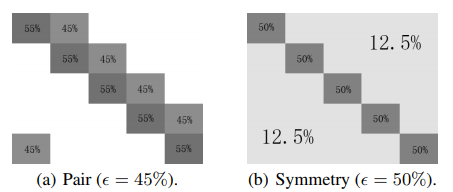
\includegraphics[scale = 0.5]{noise.png}
            \caption{Transition matrices of different noise types.}
\label{fig:noise}
\end{figure}\\
\textbf{Bing-Caltech} \cite{bing-caltech} was created with Bing and Caltech-256 datasets. The Bing dataset was formed by collecting images retrieved by Bing image search for each of the Caltech-256 category labels. Apart from the statistical differences between Bing images and Caltech images, the Bing dataset consists of rich noises, with presence of multiple objects in the same image, polysemy and caricaturization. We simply use Bing as the noisy source domain and Caltech-256 as the clean target domain. While the experiments on Office-31 and Office-Home are random noisy
data, the experiments here represent the performance in real-world weakly-supervised domain adaptation.
\subsection{Baselines}
\label{subsec:baseline}
Our approach can be used as plug in for any standard adversarial domain adaptation network. Here we use DANN\cite{dann} employed with entropy minimization on target data as a backbone. We compare our results with DANN to see how much our approach is able to improve over it. We also compare with TCL \cite{tcl} which is one of the state of the art method for WUDA. We defined two very naive variants of our approach : (1) CT-DANN-1 and (2) CT-DANN-2. In CT-DANN-1, instead of using weighting defined in equation \ref{eq:weight} we just use small loss samples as in standard co-teaching framework. We must know the noise level for CT-DANN-1 as it is the case in co-teaching too. This is a big disadvantage of this approach. In CT-DANN-2, we first train Network 1 and 2 defined in Figure \ref{fig:networks} using co-teaching framework defined in Algorithm \ref{algo:coteaching}; then only small loss source instances are used to train the DANN network. CT-DANN-2 approach is not end to end approach, however in deep learning world we like to have end to end architectures.
\subsection{Network Set-up and Optimizer}
All deep methods are implemented based on PyTorch. We use ResNet-50 pre-trained on the ImageNet dataset \cite{imagenet} as our base model, and add a fully connected bottleneck layer before its classifier layer. We fine-tune only the last residual block of the ResNet-50 model, and train the bottleneck layer, the classifier layer and the domain discriminator from scratch. The tradeoff hyper-parameter $k$ in equation \ref{eq:weight} is selected according to magnitudes of the two terms and the thresholds $(lower$ , $upper)$ in equation \ref{eq:weight} is selected according to the distribution of classifier probability values on source data i.e. $(G_{y}(G_{f}(x))$. Upper threshold is set close to 0.6 and lower threshold is set close to 0.2. Tradeoff parameters $\lambda_1$ and $\lambda_2$ defined in step 11 of Algorithm \ref{algo: ctdann} are set to be 1 and 0.1. We used mini-batch SGD with momentum of 0.9 and the same learning rate strategy as in \cite{dann}. Gradient reversal layer $(grl)$ is used in the same way as used in the DANN \cite{dann}.
\subsection{Results}
We created 3 label noise vector for source domain data for a particular noise level and noise type (Symmetric or Pairflip) while experimenting with Office 31 and Office-Home. We run all the approaches using label noise vectors generated to have fair comparison among approaches and report the average of the results on target data obtained using model trained with 3 label noise vectors for a particular approach. As Bing-Caltech dataset has native noise, so we take it as it is. We did extensive evaluation on Office 31 dataset with noise levels of 40\%, 30\% and 10\%. We expect our approach CT-DANN to perform better over DANN in case of high noise and perform almost same in case of low level noise. Experiments with 10\% level noise shows that in the case of low level noise our approach performs similarly in comparison to standard DANN. For Office-Home, we experimented with only 40\% noise. We expect the improvement on Office-Home to be in sync with improvement on Office 31.\\
Table \ref{tab:office_sym} and Table \ref{tab:office_pair} enlists the results of our approach CT-DANN in comparison with DANN and TCL on transfer tasks obtained from Office 31 dataset. It is evident that CT-DANN improves over the backbone DANN much significantly and beating the current state of the art TCL too. In case of low noise i.e. 10\%, performance of CT-DANN approach is close to DANN and TCL which is expected. 

\begin{center}
\begin{table*}[h!]
    \centering
    \begin{tabular}{|c|c|c|c|c|c|c|c|}
    \hline
    \multirow{2}{3em}{Noise Level} & \multirow{2}{4em}{Approach} &  \multicolumn{6}{|c|}{Office 31}\\
    \cline{3-8}
    & & A->D & A->W & D->A & D->W & W->A & W->D\\
    \hline
    \multirow{3}{3em}{10\%} & DANN & 87.05 & 90.94 & 69.72 & 95.58 & 67.09 & 97.42 \\
    & TCL & 88.49 & 91.10 & 67.41 & 96.54 & 67.07 & 98.33\\
    & CT-DANN & 86.50 & 92.12 & 69.73 & 98.09 & 69.50 & 99.78\\
    \hline
    \multirow{3}{3em}{30\%} & DANN & 82.26 & 83.81 & 61.42 & 82.17 & 64.27 & 87.15 \\
    & TCL & 84.56 & 88.73 & 61.42 & 82.82 & 67.15 & 92.59\\
    & CT-DANN & 87.47 & 90.18 & 64.11 & 90.66 & 69.46 & 96.94\\
    \hline
    \multirow{3}{3em}{40\%} & DANN & 73.88 & 78.99 & 60.24 & 76.17 & 54.92 & 76.79 \\
    & TCL & 86.48 & 89.35 & 60.17 & 82.29 & 56.60 & 89.79\\
    & CT-DANN & 84.47 & 90.32 & 63.80 & 86.02 & 64.58 & 92.80\\
    \hline
    \end{tabular}
    \caption{Classification Accuracy (\%) on \textbf{Office-31} with different Symmetric noise levels}
    \label{tab:office_sym}
    \end{table*}
\end{center}

\begin{center}
\begin{table*}[h!]
    \centering
    \begin{tabular}{|c|c|c|c|c|c|c|c|}
    \hline
    \multirow{2}{3em}{Noise Level} & \multirow{2}{4em}{Approach} &  \multicolumn{6}{|c|}{Office 31}\\
    \cline{3-8}
    & & A->D & A->W & D->A & D->W & W->A & W->D\\
    \hline
    
    \multirow{3}{3em}{10\%} & DANN & 86.48 & 88.23 & 69.08 & 93.74 & 70.45 & 95.36 \\
    & TCL & 87.92 & 90.18 & 65.62 & 94.91 & 68.22 & 97.34 \\
    & CT-DANN & 88.39 & 90.16 & 68.47 & 96.89 & 70.04 & 99.55 \\
    \hline
    
    \multirow{3}{3em}{30\%} & DANN & 77.59 & 74.83 & 57.69 & 73.80 & 58.61 & 79.05 \\
    & TCL & 84.25 & 85.61 & 59.99 & 76.46 & 57.51 & 84.84 \\
    & CT-DANN & 87.60 & 86.65 & 59.16 & 77.67 & 61.46 & 88.67 \\
    \hline
    
    \multirow{3}{3em}{40\%} & DANN & 62.62 & 65.36 & 47.71 & 62.89 & 49.87 & 64.88 \\
    & TCL & 71.74 & 73.03 & 46.80 & 65.16 & 50.42 & 71.89 \\
    & CT-DANN & 75.28 & 75.63 & 48.72 & 62.56 & 54.48 & 72.77 \\
    \hline
    \end{tabular}
    \caption{Classification Accuracy (\%) on \textbf{Office-31} with different Pairflip noise levels}
    \label{tab:office_pair}
    \end{table*}

\end{center}

\vspace{-1.4cm}
\begin{center}
\begin{table*}[h!]
    \centering
    \begin{tabular}{|c|c|c|c|c|c|c|c|}
    \hline
    \multirow{2}{3em}{Noise Level} & \multirow{2}{4em}{Approach} &  \multicolumn{6}{|c|}{Office 31}\\
    \cline{3-8}
    & & A->D & A->W & D->A & D->W & W->A & W->D\\
    \hline
    
    \multirow{5}{3em}{40\%} & DANN & 73.88 & 78.99 & 60.24 & 76.17 & 54.92 & 76.79 \\
    & TCL & 86.48 & 89.35 & 60.17 & 82.29 & 56.60 & 89.79\\
    & CT-DANN & 84.47 & 90.32 & 63.80 & 86.02 & 64.58 & 92.80\\
    & CT-DANN-1 & 83.85 & 90.36 & 61.67 & 85.20 & 62.55 & 90.23 \\
    & CT-DANN-2 & 81.63 & 87.08 & 59.96 & 83.72 & 64.54 & 83.98 \\
    \hline
    \end{tabular}
    \caption{Comparison with variants of CT-DANN for 40\% Symmetric noise level}
    \label{tab:office_var}
    \end{table*}
\end{center}
\vspace{-1cm}

\begin{center}
\begin{table*}[h!]
    \centering
    \resizebox{\columnwidth}{!} & DANN & 28.93 & 50.18 & 56.98 & 35.17 & 48.34 & 48.24 & 37.51 & 26.47 & 55.73 & 45.11 & 30.52 & 63.63 \\
    & TCL & 32.15 & 56.90 & 63.94 & 44.25 & 58.31 & 57.21 & 49.64 & 34.83 & 71.49 & 59.59 & 39.23 & 74.07 \\
    & CT-DANN & 35.93 & 58.99 & 66.00 & 46.32 & 58.90 & 59.08 & 49.55 & 34.97 & 69.82 & 58.63 & 40.27 & 73.64 \\
    \hline
    \end{tabular}
    }
    \caption{Classification Accuracy (\%) on \textbf{Office-Home} with 40\% Symmetric noise levels}
    \end{table*}
\end{center}

\begin{center}
\begin{table*}[h]
    \centering
    \resizebox{\columnwidth}{!} & DANN & 25.70 & 43.32 & 45.50 & 32.79 & 43.21 & 42.52 & 36.40 & 23.76 & 48.64 & 38.40 & 27.40 & 53.05 \\
    & TCL & 26.21 & 43.33 & 47.98 & 41.12 & 49.36 & 50.68 & 37.79 & 27.92 & 57.73 & 41.63 & 29.64 & 57.74 \\
    & CT-DANN & 26.35 & 43.95 & 46.90 & 39.25 & 45.97 & 48.94 & 40.30 & 29.24 & 58.65 & 42.89 & 29.49 & 58.57 \\
    \hline
    \end{tabular}
    }
    \caption{Classification Accuracy (\%) on \textbf{Office-Home} with 40\% Pairflip noise levels}
    \end{table*}
\end{center}
\vspace{-1.2cm}

\begin{center}
\begin{table*}[h]
    \centering
    \begin{tabular}{|c|c|c|}
    \hline
    {Noise} & {Approach} & {Bing-Caltech}\\
    % \cline{3-4}
    \hline
    \multirow{3}{6em}{Native Noise} & DANN & 77.28\\
    & TCL & 79.03\\
    & CT-DANN & 78.60\\
    \hline
    \end{tabular}
    \caption{Classification Accuracy (\%) on \textbf{Bing-Caltech}}
    \label{tab:bing-cal}
    \end{table*}
\end{center}
\vspace{-1.0cm}
Table \ref{tab:office_var} lists the results of CT-DANN and its variants (defined in \ref{subsec:baseline}) in comparison with DANN and TCL for 40\% noise level. Performance of CT-DANN-1 is close to CT-DANN, but there is hard assumption of knowing the noise level for CT-DANN-1. With CT-DANN-2, we were able to get improvement over backbone DANN, but it is not an end to end deep architecture and hard assumption of knowing the noise level holds in this also.\\
For Office-Home, we experimented only with 40\% noise Symmetric as well as Pairflip. We expect our approach to perform better for other noise level too as it is in Office-31.\\
Improvement over DANN for Bing-Caltech is not significant. The noise in Bing dataset consists of multiple objects in the image, caricaturization of the image.

\section{Conclusion and Future Work}
Our aim was to incorporate co-teaching framework in any standard domainadptation network. We experimented using DANN as a backbone. From experiments, It is evident improvement over DANN is quite significant. We plan to experiment with one more standard domain adaptation network also; CDAN \cite{cdan}. In this work, we experimented with label noise, but ideally our approach should work for other noise as well; noisy image or blurred image. We plan to conduct more research in the area where noise is present in the image itself or features are corrupted.   



% \color{red}
% 1. Mean with std for all 4 vectors should be sufficient rather than listing all separately.
% 2. Pairflip and symmetric noise show separately. 
% 10, 20, 30, 40, 50 percent noise - both cases 
% 3. Analysis 
% (a) No noise case - does it degrade performance?
% (b) Sequential - to show integrated algo works
% (c) Without one/both weighting - to show both weighting helps.
% (d) What is the result if we know the noise label vs. we use the proposed weighting strategy.
% Some examples of initial wrong labels and examples of small loss samples.
% - Can we compare with other approaches (maybe more recent) which they have reported?
% - Real dataset - could not find any other dataset other than Bing.
% - Another backbone.
% \color{black}





\bibliography{references}
\end{document}


























%------------------------------------------------------------------------- 
% Document starts here
% \begin{document}

% \maketitle

% \begin{abstract}
% This document demonstrates the format requirements for papers submitted
% to the British Machine Vision Conference.  The format is designed for
% easy on-screen reading, and to print well at one or two pages per sheet.
% Additional features include: pop-up annotations for
% citations~\cite{Authors06,Mermin89}; a margin ruler for reviewing; and a
% greatly simplified way of entering multiple authors and institutions.

% {\bf All authors are encouraged to read this document}, even if you have
% written many papers before.  As well as a description of the format, the
% document contains many instructions relating to formatting problems and
% errors that are common even in the work of authors who {\em have}
% written many papers before.
% \end{abstract}

% %------------------------------------------------------------------------- 
% \section{Introduction}
% \label{sec:intro}
% The proceedings of BMVC are published only in electronic form, but it is still assumed
% that readers of the papers may wish to print the paper.   This document
% illustrates the required paper format, which is designed to read well either printed
% with two pages per sheet (``2-up''), or on screen.  Note that printing with one page 
% per sheet will produce a ``large print'' version, which in many cases is not what is desired.
% To approximate the old BMVC format, print at one page per sheet, but do not choose
% the option to ``scale to fit paper''.

% \LaTeX\ users should use this template in order to prepare their paper.
% Users of other packages should emulate the style and layout of this
% example.  Note that best results will be achieved using {\tt pdflatex},
% which is available in most modern distributions.

% \subsection{Paper length: nine pages plus bibliography}
% Paper length should not exceed 9~pages, {\em not counting} the bibliography.  {\bf Papers which are
%  overlength will not be reviewed}.  This includes papers where the
% margins and formatting are deemed to have been significantly altered from
% those laid down by this style guide.  The reason such papers will not be
% reviewed is that there is no provision for supervised revisions of
% manuscripts.  The reviewing process cannot determine the suitability of the
% paper for presentation in nine pages if it is reviewed in twelve.

% The bibliography should begin immediately after the paper text.  It may
% be of any length, within reason.  It should {\em not} include
% annotations, figures, or any other paraphernalia intended to subvert the
% paper length requirement.

% \begin{figure}
% \begin{tabular}{ccc}
% \bmvaHangBox{\fbox{\parbox{2.7cm}{~\\[2.8mm]
% \rule{0pt}{1ex}\hspace{2.24mm}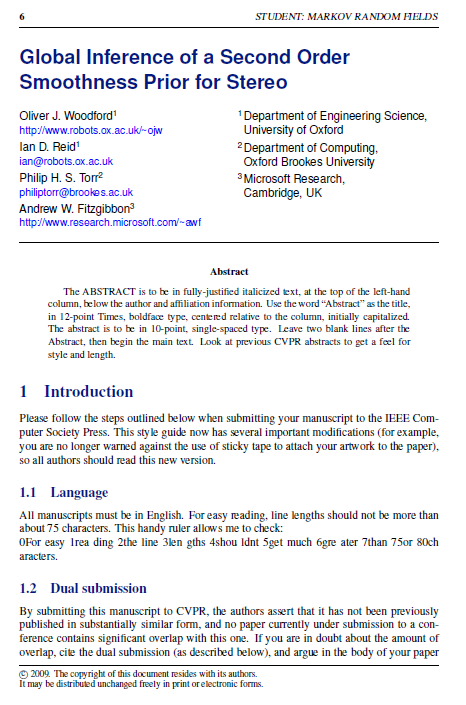
\includegraphics[width=2.33cm]{images/eg1_largeprint.png}\\[-0.1pt]}}}&
% \bmvaHangBox{\fbox{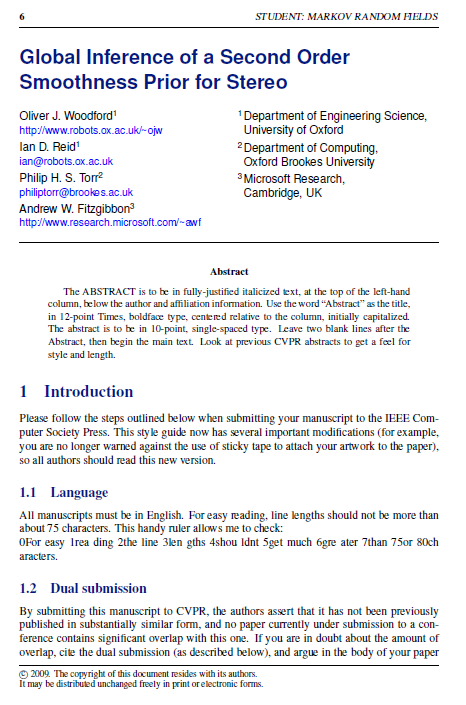
\includegraphics[width=2.8cm]{images/eg1_largeprint.png}}}&
% \bmvaHangBox{\fbox{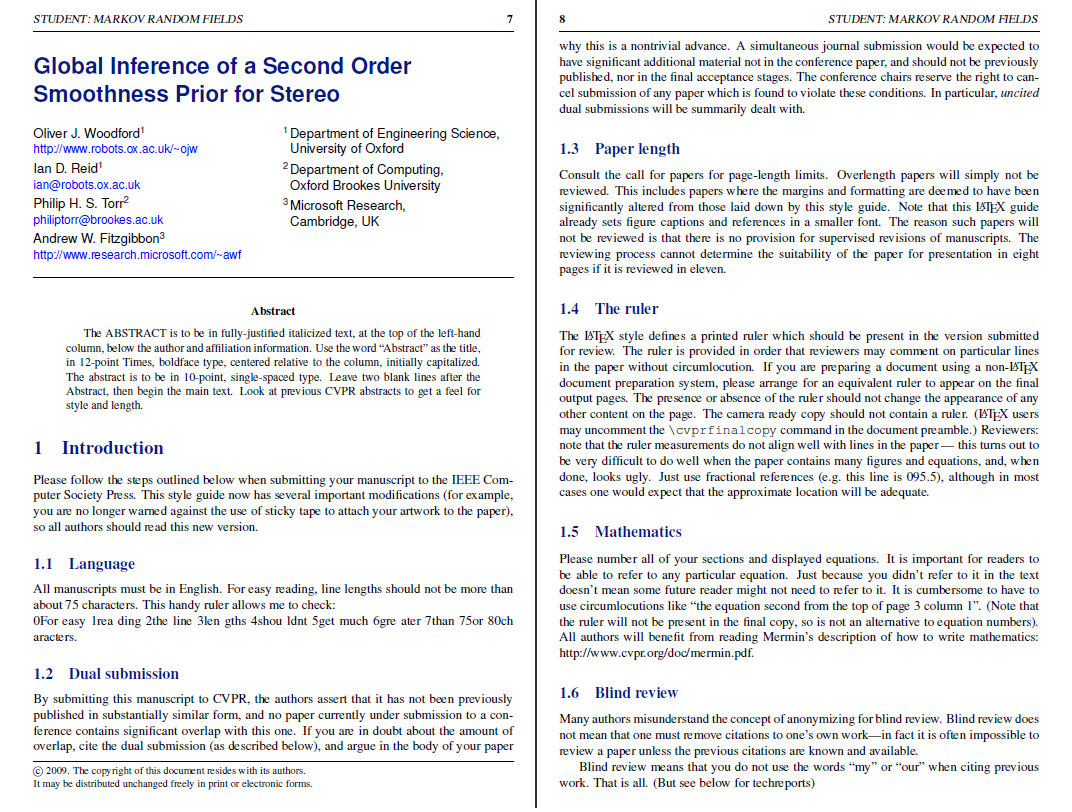
\includegraphics[width=5.6cm]{images/eg1_2up.png}}}\\
% (a)&(b)&(c)
% \end{tabular}
% \caption{It is often a good idea for the first figure to attempt to
% encapsulate the article, complementing the abstract.  This figure illustrates
% the various print and on-screen layouts for which this paper format has
% been optimized: (a) traditional BMVC print format; (b) on-screen
% single-column format, or large-print paper; (c) full-screen two column, or
% 2-up printing. }
% \label{fig:teaser}
% \end{figure}

% \subsection{Citations}
% When citing a multi-author paper, you may save space by using ``{\em et
% alia}'', shortened to ``\etal'' (not ``{\em et.\ al.}'' as ``{\em et}'' is
% a complete word.)  The provided \verb'\etal' macro is a useful {\em aide
% memoire} in this regard.  However, use it only when there are three or more
% authors.  Thus, the following is correct: `` Frobnication has been trendy
% lately.  It was introduced by Alpher~\cite{Alpher02}, and subsequently
% developed by Alpher and Fotheringham-Smythe~\cite{Alpher03}, and Alpher
% \etal~\cite{Alpher04}.''

% This is incorrect: ``... subsequently developed by Alpher \etal~\cite{Alpher03} ...''
% because reference~\cite{Alpher03} has just two authors.  If you use the
% \verb'\etal' macro, then you need not worry about double periods
% when used at the end of a sentence as in Alpher \etal.

% %For this citation style, keep multiple citations in numerical (not
% %chronological) order, so prefer
% We use {\tt natbib}, so citations in random order are nicely sorted:
%  \cite{Alpher03,Alpher02,Authors06b,Authors06}.  However, we don't use the
% compress option, as we want each reference to have its own hyperlink and
% popup window.

% %------------------------------------------------------------------------- 
% \subsection{Footnotes}

% Please use footnotes\footnote {This is what a footnote looks like.  It
% often distracts the reader from the main flow of the argument.} sparingly.
% Indeed, try to avoid footnotes altogether and include necessary peripheral
% observations in 
% the text (within parentheses, if you prefer, as in this sentence).  If you
% wish to use a footnote, place it at the bottom of the column on the page on
% which it is referenced. Use Times 8-point type, single-spaced.


% \begin{figure*}
% \begin{center}
% \fbox{\rule{0pt}{2in} \rule{.9\linewidth}{0pt}}
% \end{center}
%   \caption{Example of a short caption, which should be centered.}
% \label{fig:short}
% \end{figure*}

% \begin{table}
% \begin{center}
% \begin{tabular}{|l|c|}
% \hline
% Method & Frobnability \\
% \hline\hline
% Theirs & Frumpy \\
% Yours & Frobbly \\
% Ours & Makes one's heart Frob\\
% \hline
% \end{tabular}
% \end{center}
% \caption{Results.   Ours is better.}
% \end{table}

% \subsection{Mathematics}

% Please number all of your sections and displayed equations.  It is
% important for readers to be able to refer to any particular equation.  Just
% because you didn't refer to it in the text doesn't mean some future reader
% might not need to refer to it.  It is cumbersome to have to use
% circumlocutions like ``the equation second from the top of page 3 column
% 1''.  (Note that the ruler will not be present in the final copy, so is not
% an alternative to equation numbers).  All authors will benefit from reading
% Mermin's description~\cite{Mermin89} of how to write mathematics.


% %------------------------------------------------------------------------- 
% \subsection{References}

% List and number all bibliographical references in 9-point Times,
% single-spaced, at the end of your paper. When referenced in the text,
% enclose the citation number in square brackets, for
% example~\cite{Authors06}.  Where appropriate, include the name(s) of
% editors of referenced books.


% %------------------------------------------------------------------------
% \subsection{Color}

% Color is valuable, and will be visible to readers of the electronic copy.
% However ensure that, when printed on a monochrome printer, no important
% information is lost by the conversion to grayscale.

% \bibliography{egbib}
% \end{document}